\chapter{Anhang}
\section{Liste bestehender Rails 2/3 Web Content Management Systeme bzw. Blogging-Software}
\begin{table}[!ht]
\center
\begin{tabular}[]{|p{3cm}|p{8cm}|p{4cm}|}
% Begin Rails 2
\hline
\multicolumn{3}{|p{15cm}|}{\textbf{OpenSource Web Content Management Systeme mit Rails 2.x Unterstützung}}\\
\hline
\textbf{Projektname}&\textbf{Projektseite im Internet}&\textbf{Aktive Weiterentwicklung}\\
\hline
adva-cms & \href{https://github.com/svenfuchs/adva\_cms}{https://github.com/svenfuchs/adva\_cms} & Ja \\
\hline
\cellcolor{alicegrey} Alchemy CMS & \cellcolor{alicegrey} \href{http://magiclabs.github.com/alchemy/}{http://magiclabs.github.com/alchemy/} & \cellcolor{alicegrey} Ja \\
\hline
Ansuz CMS & \href{https://github.com/knewter/ansuz}{https://github.com/knewter/ansuz} & eingestellt\\
\hline
Casein & \href{http://www.caseincms.com/}{http://www.caseincms.com/} & Ja \\
\hline
Comatose & \href{http://comatose.rubyforge.org/}{http://comatose.rubyforge.org/} & eingestellt\\
\hline
Compages & \href{http://compages.wordpress.com/}{http://compages.wordpress.com/} & eingestellt\\
\hline
Geego CMS & \href{http://gitorious.org/geego-cms\#more}{http://gitorious.org/geego-cms\#more} & eingestellt\\
\hline
Mephisto & \href{https://github.com/halorgium/mephisto}{https://github.com/halorgium/mephisto} & eingestellt\\
\hline
Radiant & \href{http://radiantcms.org/}{http://radiantcms.org/} & Ja \\
\hline
Railfrog & \href{http://railfrog.com/}{http://railfrog.com/} & Nein \\
\hline
Rojo CMS & \href{https://github.com/onomojo/rojo}{https://github.com/onomojo/rojo} & unbekannt\\
\hline
Rubricks & \href{http://rubricks.org/}{http://rubricks.org/} & eingestellt\\
\hline
Skyline CMS & \href{http://www.skylinecms.nl/}{http://www.skylinecms.nl/} & Ja \\
\hline
Station & \href{https://github.com/atd/station}{https://github.com/atd/station} & Ja\\
\hline
Typhus & \href{http://typus.heroku.com/}{http://typus.heroku.com/} & eingestellt\\
\hline
Vrame & \href{https://github.com/9elements/vrame}{https://github.com/9elements/vrame} & eingestellt\\
\hline
Webiva & \href{http://webiva.org/}{http://webiva.org/} & Ja \\
\hline
zenacms & \href{http://zenadmin.org/}{http://zenadmin.org/} & Ja \\
\hline
\end{tabular}
\end{table}

% Begin Rails 3
\begin{table}
\center
\addtocounter{footnote}{1}
\begin{tabular}[]{|p{3cm}|p{8cm}|p{4cm}|}
\hline
\multicolumn{3}{|p{15cm}|}{\textbf{Open Source Web Content Management Systeme mit Rails 3.x Unterstützung}}\\
\hline
\textbf{Projektname}&\textbf{Projektseite im Internet}&\textbf{Aktive Weiterentwicklung}\\
\hline
adva-cms2 & \href{https://github.com/svenfuchs/adva-cms2}{https://github.com/svenfuchs/adva-cms2} & Ja \\
\hline
\cellcolor{alicegrey}Alchemy CMS & \cellcolor{alicegrey} \href{http://magiclabs.github.com/alchemy/}{http://magiclabs.github.com/alchemy/} &\cellcolor{alicegrey} Ja \\
\hline
\cellcolor{alicegrey}Browser CMS & \cellcolor{alicegrey} \href{http://browsercms.org}{http://browsercms.org} & \cellcolor{alicegrey} Ja \\
\hline
Casein & \href{https://github.com/spoiledmilk/casein3}{https://github.com/spoiledmilk/casein3} & Ja \\
\hline
Comfortable Mexican Sofa & \href{https://github.com/twg/comfortable-mexican-sofa}{https://github.com/twg/comfortable-mexican-sofa} & ja  \\
\hline
\cellcolor{alicegrey} Locomotive CMS & \cellcolor{alicegrey} \href{http://www.locomotivecms.com/}{http://www.locomotivecms.com/} & \cellcolor{alicegrey} Ja \\
\hline
Nesta CMS & \href{https://github.com/gma/nesta}{https://github.com/gma/nesta} & ja  \\
\hline
\cellcolor{alicegrey} Refinery CMS & \cellcolor{alicegrey} \href{http://refinerycms.com/}{http://refinerycms.com/} & \cellcolor{alicegrey} Ja \\
\hline
Surtout CMS & \href{http://surtoutcms.com/}{http://surtoutcms.com/} & noch nicht veröffentlicht \\
\hline
typo (Blogging) & \href{http://fdv.github.com/typo/}{http://fdv.github.com/typo/} & Ja \\
\hline
% End Rails 3
\end{tabular}
\end{table}
\begin{comment}
% begin closed source
\begin{table}
\center
\begin{tabular}[]{|p{3cm}|p{8cm}|p{4cm}|}
\hline
\multicolumn{3}{|p{15cm}|}{\textbf{Closed Source Web Content Management Systeme mit Rails 3.x Unterstützung}}\\
\hline
\textbf{Projektname}&\textbf{Projektseite im Internet}&\textbf{Aktive Weiterentwicklung}\\
\hline
Blocks & \href{http://www.blocksglobal.com/}{http://www.blocksglobal.com/} & Ja \\
\hline
% End clsoed source
\end{tabular}
\end{table}
\end{comment}
\section{Funktionsübersicht der untersuchten Rails WCMS}
Die Ergebnisse der durchgeführten funktionalen Analyse (Kaiptel \ref{sec:durchanalyse}) werden im Folgenden für jedes System noch einmal separat in einer Übersicht zusammengefasst:


\subsubsection{Alchemy CMS}

\begin{description}
\item[\emph{Erstellung}]\mbox{~}\\*
\begin{itemize}
	\item Umfassende Möglichkeiten zur Erstellung und Verwaltung von Seiten und verschiedenen Inhaltselementen in verschiedenen Sprachen
	\item Template-Erstellung und -verwaltung findet im Quellcode der Rails-Anwendung statt
	\item Umsetzung komplexer Seitenlayouts möglich
\end{itemize}
\item[\emph{Kontrolle}]\mbox{~}\\*
\begin{itemize}
	\item eingeschränkte Rechteverwaltung mit festgelegten Gruppen für Front- und Backend (Registriert, Author, Redakteur, Administrator)
	\item kein umfassendes Linkmanagement
\end{itemize}
\item[\emph{Freigabe}]\mbox{~}\\*
\begin{itemize}
	\item Einfacher Freigabeprozess für Internetseiten und Inhalte
	\item keine umfassende Workflowfunktionalität
\end{itemize}
\item[\emph{Publikation}]\mbox{~}\\*
\begin{itemize}
	\item Trennung der Inhalte vom Design durch Verwendung von Templates
	\item umfassende Seiten- und Inhaltsverwaltung mit Möglichkeiten zum Kopieren und Verschieben der Inhalte (Zwischenablagefunktion)
\end{itemize}
\item[\emph{Terminierung/Archivierung}]\mbox{~}\\*
\begin{itemize}
	\item Seiten und Inhalte können nicht archiviert oder zeitraumgebunden veröffentlicht werden
\end{itemize}
\end{description}

\newpage
\subsubsection{Browser CMS}

\begin{description}
\item[\emph{Erstellung}]\mbox{~}\\*
\begin{itemize}
	\item Umfassende Möglichkeiten zur Erstellung und Verwaltung von einsprachigen Seiten und verschiedenen Inhaltselementen
	\item Template-Erstellung und -verwaltung im Backend der Anwendung
	\item Umsetzung komplexer Seitenlayouts möglich
\end{itemize}
\item[\emph{Kontrolle}]\mbox{~}\\*
\begin{itemize}
	\item Rechteverwaltung mit vordefinierten Gruppen für Front- und Backend sowie Möglichkeiten zum Erstellen eigener Gruppen
	\item kein umfassendes Linkmanagement
\end{itemize}
\item[\emph{Freigabe}]\mbox{~}\\*
\begin{itemize}
	\item Einfacher Freigabeprozess für Internetseiten und Inhalte
	\item keine umfassende Workflowfunktionalität
\end{itemize}
\item[\emph{Publikation}]\mbox{~}\\*
\begin{itemize}
	\item Trennung der Inhalte vom Design durch Verwendung verschiedener Template-Sprachen
	\item Wiederverwendung von Inhaltenselementen
\end{itemize}
\item[\emph{Terminierung/Archivierung}]\mbox{~}\\*
\begin{itemize}
	\item Archivierung von erstellten Seiten
	\item keine zeitraumgebundene Veröffentlichung von Seiten und Inhalten möglich
\end{itemize}
\end{description}


\newpage
\subsubsection{Locomotive CMS}

\begin{description}
\item[\emph{Erstellung}]\mbox{~}\\*
\begin{itemize}
	\item Umfassende Möglichkeiten zur Erstellung und Verwaltung von einsprachigen Seiten und verschiedenen Inhaltselementen
	\item Inhaltselemente können im Backend der Seite individuell erstellt werden
	\item Umsetzung komplexe Layouts mit verschiedenen Seiten- und Inhaltselementen möglich
\end{itemize}
\item[\emph{Kontrolle}]\mbox{~}\\*
\begin{itemize}
	\item eingeschränkte Rechteverwaltung mit vordefinierten Gruppen für das Backend
	\item kein umfassendes Linkmanagement
\end{itemize}
\item[\emph{Freigabe}]\mbox{~}\\*
\begin{itemize}
	\item keine Abbildung von Freigabeprozessen für Internetseiten und Inhalte möglich
	\item keine Workflowfunktionalität
\end{itemize}
\item[\emph{Publikation}]\mbox{~}\\*
\begin{itemize}
	\item Trennung der Inhalte vom Design durch Verwendung der Template-Sprache Liquid
	\item Wiederverwendung von Inhaltenselementen
	\item eingeschränkte Möglichkeiten zum Verschieben von Seiten und Inhalten
\end{itemize}
\item[\emph{Terminierung/Archivierung}]\mbox{~}\\*
\begin{itemize}
	\item Archivierung und Terminierung von Inhalten und Seiten ist nicht möglich
\end{itemize}
\end{description}

\subsubsection{Refinery CMS}

\begin{description}
\item[\emph{Erstellung}]\mbox{~}\\*
\begin{itemize}
	\item Erstellung und Verwaltung von mehrsprachigen Seiten und Inhaltsböcken
	\item Inhaltselemente können im Backend der Seite individuell erstellt werden
	\item Umsetzung komplexe Layouts mit Hilfe von Rails Views möglich
\end{itemize}
\item[\emph{Kontrolle}]\mbox{~}\\*
\begin{itemize}
	\item keine Rechteverwaltung für Seiten, Inhalte und Nutzer
	\item kein umfassendes Linkmanagement
\end{itemize}
\item[\emph{Freigabe}]\mbox{~}\\*
\begin{itemize}
	\item keine Unterstützung von Freigabeprozessen
	\item Erstellte Seiten können in den Bearbeitungsmodus gesetzt werden  und sind dadurch nicht mehr erreichbar
	\item keine Workflowfunktionalität
\end{itemize}
\item[\emph{Publikation}]\mbox{~}\\*
\begin{itemize}
	\item Trennung der Inhalte vom Design durch Verwendung der in Rails üblichen ERB-Views
	\item keine Wiederverwendung von Inhaltenselementen möglich
	\item keine Möglichkeiten zum Verschieben und Kopieren von Inhalten
\end{itemize}
\item[\emph{Terminierung/Archivierung}]\mbox{~}\\*
\begin{itemize}
	\item Archivierung und Terminierung von Inhalten und Seiten ist nicht möglich
\end{itemize}
\end{description}





\section{Crudify-Methode von Refinery CMS 1.0.8}
\lstinputlisting[label=crudify, nolol=true, title=Implementierung der Crudify-Methode in Refinery CMS 1.0.8,language=Ruby]{code/crudify_method.rb}
\newpage
\section{Ext-Direct Spezifikation für Ext Js 3.0}
Im folgenden Abschnitt wird die offizielle PDF-Version der Ext Js 3.0-Spezifikation als PDF-Version abgebildet. Die Formatierung und Gestaltung entspricht dabei der originalen PDF-Version vom 25.Oktober 2011. Zum Zeitpunkt der Veröffentlichung dieser Arbeit existierth keine Spezifikation für die neuste Version 4.x der Ext Js-Bibliothek.
\label{extspec}
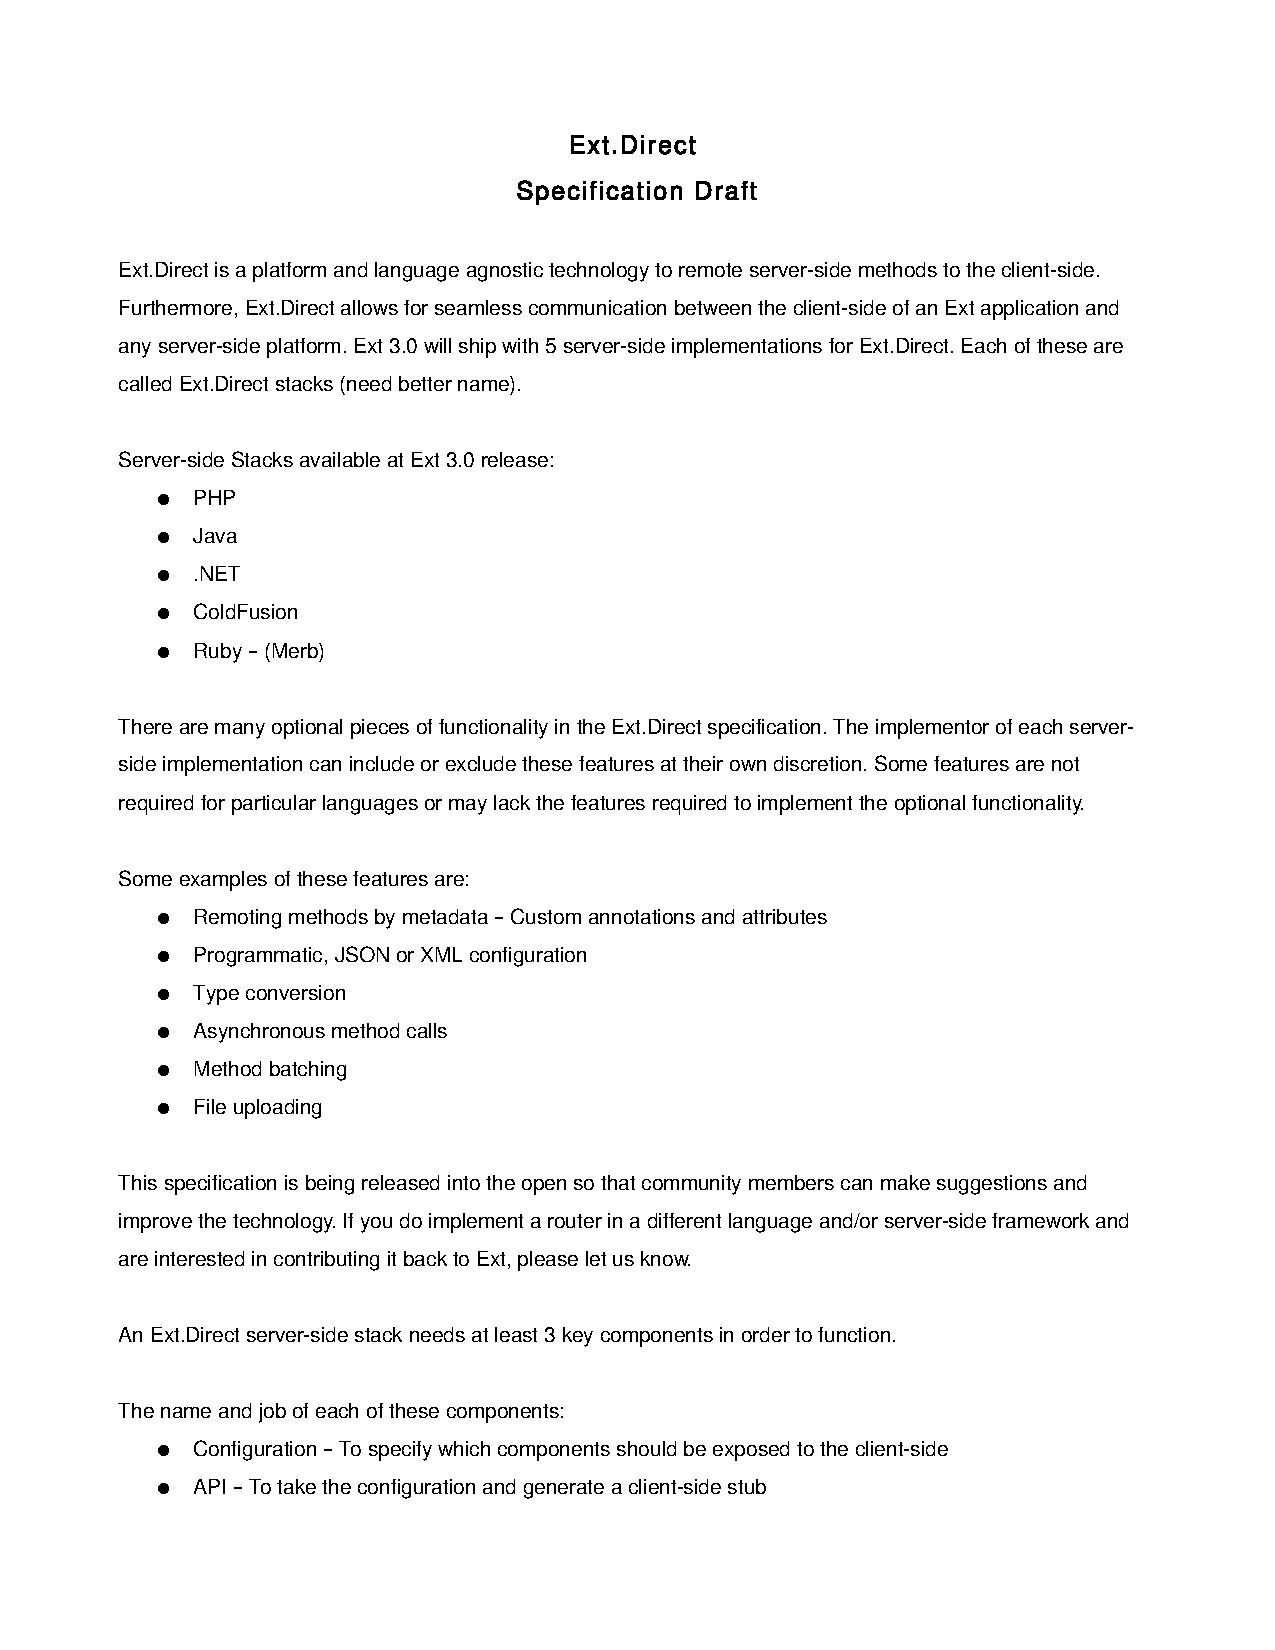
\includepdf{pdf/extdirect.pdf}
\section{Nutzung von Extr in einer Rails 3.1-Anwendung}
Im folgenden Abschnitt wird die Installation und Nutzung des erstellten Plugins Extr in einer neu erstellten Rails 3-Anwendung demonstriert. Das erstellte Paket ist noch in der Entwicklungsphase und konnte nicht vollständig auf seine Sicherheit überprüft werden\footnote{Sicherheitsbedenken in den Bereichen CSRF und XSS wurden bei der Vorstellung des Paktes aufgezeigt.}. Der Quellcode der Anwendung kann unter folgender Adresse heruntergeladen werden:
Extr: \href{https://github.com/skeller1/extr}{https://github.com/skeller1/extr}
Für die folgenden Beschreibungen wird eine funktionsbereite Rails 3.1-Installation vorausgesetzt.
\begin{enumerate}
\item
Erstellung einer neuen Rails 3-Anwendung \emph{directtest}
\begin{lstlisting}[frame=single, numbers=none]
rails new directtest
\end{lstlisting}
\item
Aktivierung des Plugins/Gems in der Gemfile der erstellten Rails-Anwendung

\begin{lstlisting}[frame=single, numbers=none]

# ...
gem "extr", :git => "git://github.com/skeller1/extr.git"
# ...

\end{lstlisting}

\item
Erstellung einer Rails 3 Standard-Ressource Projekt und Erzeugung der notwendigen Datenbanktabelle.

\begin{lstlisting}[frame=single, numbers=none]
rails g scaffold project name:string description:text
rake db:migrate
\end{lstlisting}

\item
Einbinden der notwendigen Ext-Direct-Bibliotheken mit Hilfe der vom Plugin zur Verfügung gestellten Helfermethoden (View Helpers). Der Namensraum des Ext-Direct-Provider ist \emph{Rails}.

\begin{lstlisting}[language=xml,frame=single,title=\emph{app/views/layouts/application.html.erb}, numbers=none]
<!DOCTYPE html>
<html>
<head>
  <title>Extr</title>
  <%= stylesheet_link_tag "extr/application" %>
  <%= javascript_include_tag "extr/application" %>
  <%= csrf_meta_tags %>
  <%= ext_base_tag %>
  <%= ext %>
  <%= ext_direct_provider "Rails" %>
</head>
<body>
    <%= yield %>
</body>
</html>
\end{lstlisting}

\item
Registrierung der Ext-Direct-fähigen Controller-Methoden (Actions) im Projekte-Controller (projects controller). Die erstellten Methoden sind nur als Beispiel zu verstehen und können entsprechend angepasst werden.

\begin{lstlisting}[language=ruby,frame=single,title=\emph{app/controllers/projects\_controller.rb}, numbers=none]
class ProjectsController < ApplicationController

  # activate extr for this controller
  include Extr::DirectController


  #disable Rails 3 authenticity_token for demonstration, not recom. in production
  skip_before_filter :verify_authenticity_token


  #register 2 ext direct controller action with different, optional controller name (MyDirectController)
  direct "MyDirectController",
    :getChildProject => 1,
    :someOtherMethod => 2


  def getChildProject
    # render a random project name as json response
    render :json => {:name => "Project#{Random.rand(11)}"}.to_json
  end

\end{lstlisting}

\item
Im Index-HTML-View der Projekt-Ressource (http://localhost:3000/projects) kann nun durch einen Javascript-Aufruf eine Anfrage an die registrierten Ext-Direct-Controller-Methoden gesendet werden. Abbildung \ref{extrreqeust} zeigt das Ergebnis eines mit Hilfe des Mozilla Firefox Plugins Firebug temporär ausgeführten JavaScript-Codes.
Als Javascript-Callback wird der Name des Projektes zurückgegeben (\emph{Project9}).
\begin{lstlisting}[language=ruby,frame=single,title=\emph{Javascript zum Aufruf des Projekt-Controllers in der Rails-Anwendung}]
Rails.MyDirectController.getChildProject("param",function(r,e){
 alert(r.name);
});

\end{lstlisting}

\begin{figure}[!h]
\begin{center}
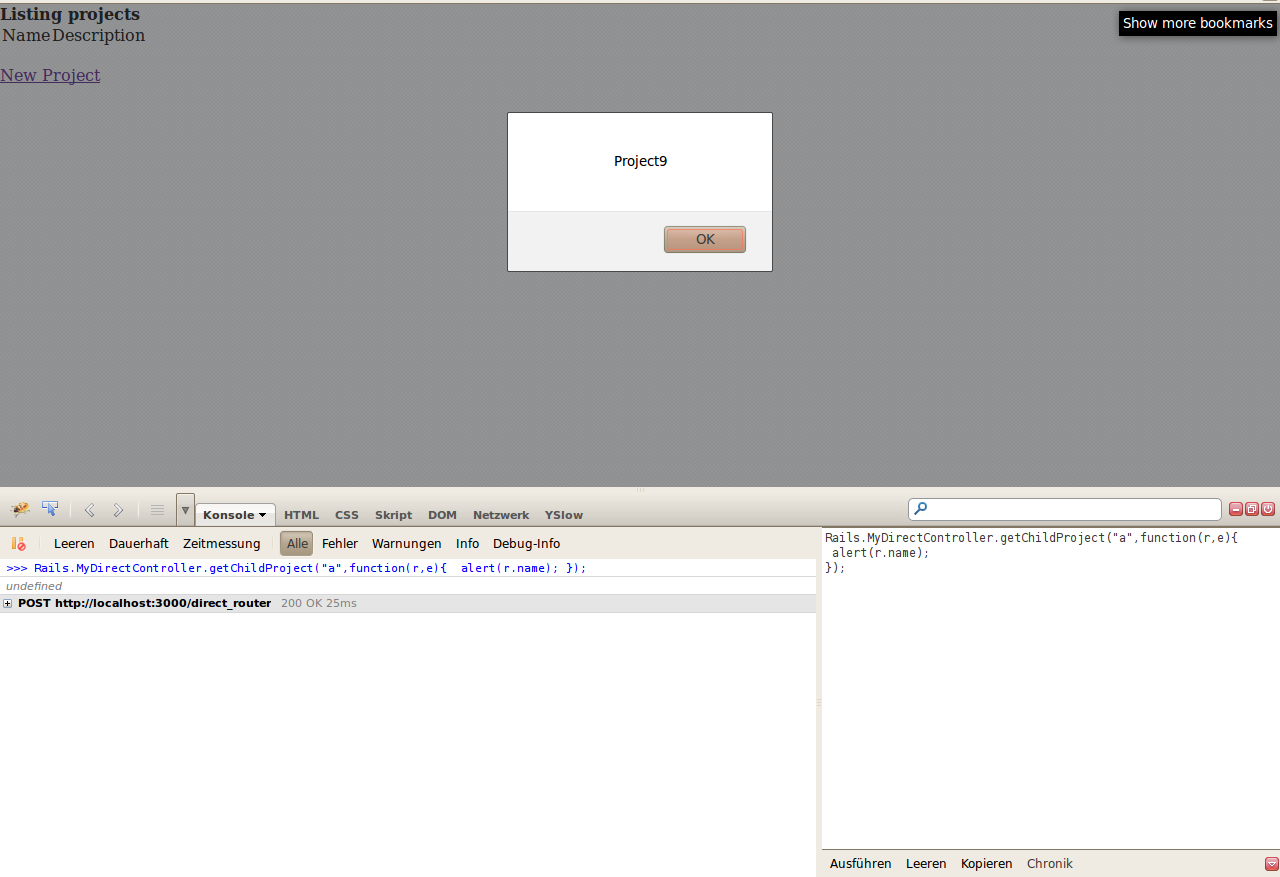
\includegraphics[scale=0.4]{images/anhang/extrbrowserrequest.png}
\caption{Mit Hilfe von Firebug formulierte Javascript-Ext-Direct-Anfrage mit ausgegebener Antwort der Rails-Anwendung}
\label{extrreqeust}
\end{center}
\end{figure}
\end{enumerate}

%\section{Java Content Repository Spezifikation}
%
\includepdf{pdf/jcr-spec.pdf}

